\documentclass{article}
\usepackage{import}
\usepackage{amsmath}
\usepackage{tabularray}
\usepackage{float}


\import{lib/latex/}{wgmlgz}
\patchcmd{\thebibliography}{\section*}{\section}{}{}

\begin{document}
\itmo[
      variant=13,
      labn=2,
      discipline=Вычислительная математика,
      group=P3212,
      student=Соколов Анатолий Владимирович,
      teacher=Наумова Надежда Александровна 
]
\lstset{language=rust}
\newgeometry{
  a4paper,
  top=20mm,
  right=10mm,
  bottom=20mm,
  left=30mm
}
\tableofcontents

\section{Задание}
% \begin{enumerate}
      Вычислительная часть лабораторной работы должна быть представлена в виде таблиц и отображена только в отчете.
      \begin{enumerate}
            \item Отделить корни заданного нелинейного уравнения графически (вид уравнения представлен в табл. 2.6)
            \item График исследуемой функции отобразить в отчете
            \item Определить интервалы изоляции корней
            \item Уточнить корни заданного нелинейного уравнения с точностью $\varepsilon=10^{-2}$
            \item Используемые методы для уточнения каждого из трех корней многочлена представлены в табл. 2.7
            \item Вычисления оформить в виде таблиц (табл. 2.1–2.5), в зависимости от заданного метода. Для всех значений в таблицах удержать 3 знака после запятой;
      \end{enumerate}
      \begin{table}[h!]
            \centering
            \begin{tabular}{|l|l|l|l|l|}
            \hline
            \textbf{№ шага} & $x_k$ & $x_{k+1}$ & $f(x_k+1)$ & $|x_k - x_{k+1}|$ \\ \hline
            1 & & & &                \\ \hline
            2 & & & &                \\ \hline
            3 & & & &                \\ \hline
            ... & & & &                \\ \hline
            \end{tabular}
            \caption{Уточнение корня уравнения методом простой итерации}
            \label{table:functional_requirements}
        \end{table}

\subsection{Вариант}

\subsection{Для нелинейных уравнений должно быть реализовано}

\begin{enumerate}
      \item Все численные методы (см. табл. 2.8) должны быть реализованы в виде класса /метода/функции;
      \item Пользователь выбирает уравнение, корень/корни которого требуется вычислить (3–5 функций, в том числе и трансцендентные), из тех, которые предлагает программа;
      \item Предусмотреть ввод исходных данных (границы интервала, погрешность вычисления) из файла или с клавиатуры по выбору конечного пользователя;
      \item Организовать вывод графика функции на исследуемом интервале (с запасом);
      \item Выполнить верификацию исходных данных. Необходимо анализировать наличие корня на введенном интервале. Если на интервале несколько корней или они отсутствуют – выдавать соответствующее сообщение. Программа должна реагировать на некорректные введенные данные;
      \item Для методов, требующих начальное приближение к корню (методы Ньютона, секущих, хорд с фиксированным концом, простой итерации), выбор начального приближения (а или b) вычислять в программе;
      \item Для метода простой итерации проверять достаточное условие сходимости метода на введенном интервале. Если оно не выполняется, выводить соответствующее сообщение. При этом попытаться решить нелинейное уравнение, ограничив итерационный процесс заданным в программе максимальным числом итераций;
      \item Для каждого метода учитывать все критерии выхода из итерационного цикла. Проверить, как изменятся результаты, если учитывать либо критерии по аргументу, либо критерии по функции;
      \item Предусмотреть вывод результатов (найденный корень уравнения, значение функции в корне, число итераций) в файл или на экран по выбору конечного пользователя;
      \item Проанализировать полученные результаты, оценить точность решения задачи;
      \item Программа должна быть протестирована на различных наборах данных, в том числе и некорректных.
\end{enumerate}

\subsection{Для систем нелинейных уравнений должно быть реализовано}

\begin{enumerate}
      \item Пользователь выбирает предлагаемые программой системы двух нелинейных уравнений (2–3 системы);
      \item Организовать вывод графика функций.
      \item Ввести начальные приближения с клавиатуры;
      \item Для метода простой итерации проверить достаточное условие сходимости. Если оно не выполняется, выводить соответствующее сообщение. При этом попытаться решить систему нелинейных уравнений, ограничив итерационный процесс заданным в программе максимальным числом итераций;
      \item Организовать вывод вектора неизвестных: ;
      \item Организовать вывод количества итераций, за которое было найдено решение;
      \item Организовать вывод вектора погрешностей: ;
      \item Проверить правильность решения системы нелинейных уравнений.
      \item Программа должна быть протестирована при различных наборах данных, в том числе и некорректных.
\end{enumerate}

\subsection{Варианты задания}
      $$x^3+4.81x^2-17.37x+5.38$$
      \\
      \textbf{Выбор метода для вычислительной реализации задачи}
      \\
      Метод простой итерации
      \\
      \textbf{Выбор метода для программной реализации задачи}
      \\
      Решение нелинейных уравнений: метод половинного деления, метод Ньютона, метод простой итерации
      \\
      Решение систем нелинейных уравнений: метод Ньютона.
\subsection{Цель работы}
      Изучить численные методы решения нелинейных уравнений и их систем, найти корни заданного нелинейного уравнения/системы нелинейных уравнений, выполнить программную реализацию методов.

\section{Выполнение}

\subsection{Блок-схема реализованного алгоритма}
      % 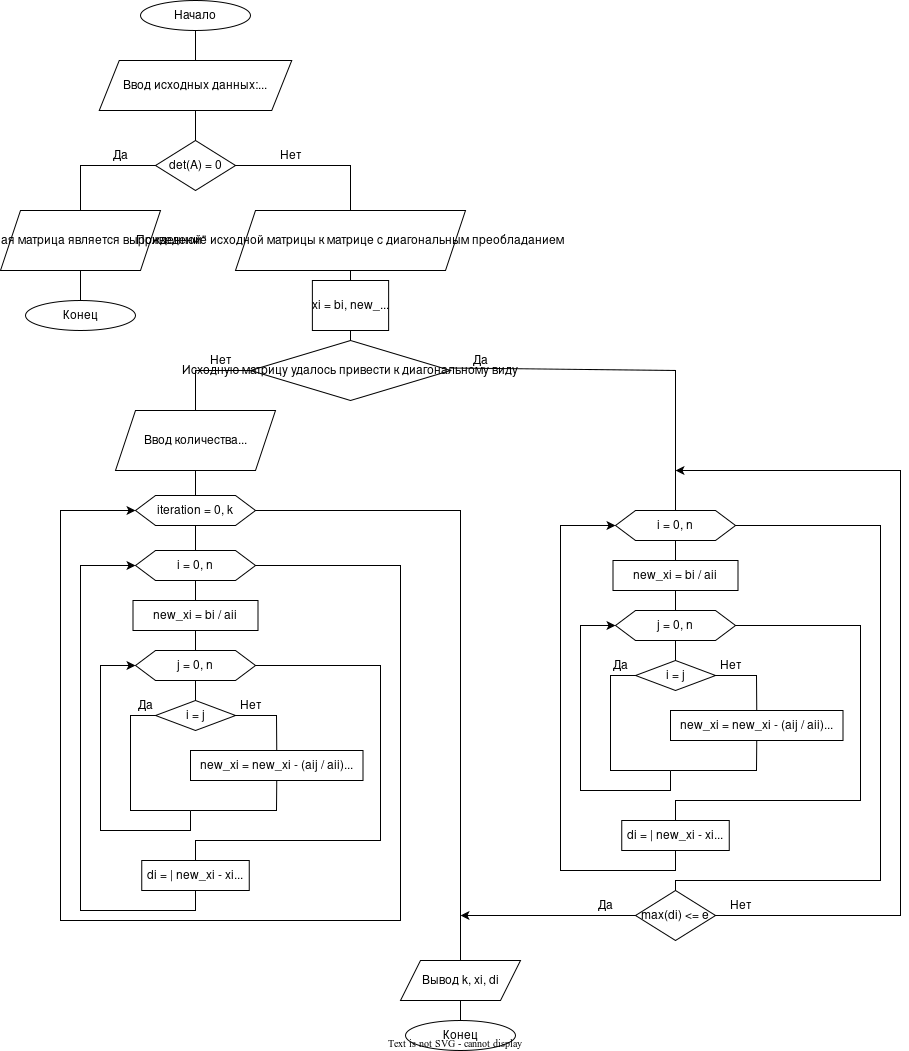
\includegraphics[scale=0.5]{AlgoSheme.png}
\subsection{Ссылка на GitHub c основной реализацией}
      \href{https://github.com/isofinly/compmath}{Github}

\subsection{Примеры и результаты работы программы}
      \begin{center}

      \end{center}
      

\section{Заключение}
Я познакомился с новым для меня и крайне необыкновенным вычислением СЛАУ на языке rust.


\begin{thebibliography}{9}
    \bibitem{Методичка}Слайды с лекций (2023). // Кафедра информатики и вычислительной техники -- Малышева Татьяна Алексеевна, к.т.н., доцент.
\end{thebibliography} 

\end{document}
